\begin{frame}[ctb!]
\frametitle{Thermal Modeling in Cyder}
Two types of thermal modeling occur in Cyder. 
\begin{itemize}
\item The first is \textbf{capacity estimation} for waste stream acceptance.
\item The next is \textbf{heat evolution} which (optionally) determines heat evolution in 
the modules over repository lifetime.
\end{itemize}
\end{frame}

\begin{frame}
\frametitle{Thermal Modeling in Cyder}
Each can be acheived with one thermal model,
\begin{itemize}
\item This model employs a Specific Temperature Change algorithm \cite{radel_effect_2007, radel_repository_2007} and
\item relies on a supporting \textbf{response database} combining detailed 
spent nuclear fuel composition data \cite{carter_fuel_2011} with a detailed 
thermal repository performance analysis tool from Lawrence Livermore National 
Lab (LLNL) and the Used Fuel Disposition (UFD) 
campaign \cite{greenberg_application_2012}.  
\end{itemize}
\end{frame}
\begin{frame}
\frametitle{Thermal Modeling in Cyder}
This method is capable of rapid estimation of temperature increase near emplacement tunnels as a function of 
\begin{itemize}
\item waste composition,
\item limiting radius, $r_{lim}$, 
\item waste package spacing, $S$, 
\item near field thermal conductivity, $K_{th}$, 
\item and near field thermal diffusivity, $\alpha_{th}$.
\end{itemize}
\end{frame}




\subsubsection{Specific Temperature Change Method}
Introduced by Radel, Wilson et. al., the Specific Temperature Change method uses 
a linear approximation to arrive at the thermal loading density limit.  
When the thermal time constant of the rock is much shorter than the waste form 
decay package, the change in package wall temperature can be described by 

\begin{align}
\Delta T_1 &= q(t_0)\rho_{limit}C'
\intertext{where}
\Delta T_1 &= T_{lim} - T_{amb} \nonumber\\
T_{lim} &= \mbox{ Temperature limit }[^{\circ}C]\nonumber\\
T_{amb} &= \mbox{ Ambient rock temperature }[^{\circ}C]\nonumber\\
q(t_0) &= \mbox{ Heat at the inital time} \nonumber \\
\rho_{limit} &= \frac{C_1}{Q_1}\nonumber\\
C' &= \mbox{ Thermal constant }[-]\nonumber\\
\Delta T &= T_{lim}-T_{amb}[^{\circ}C]\nonumber\\
\end{align}

Figure \ref{fig:CmScaling} demonstrates the scaling of an STC curve to represent 
the heat from $25.9g$ of initial $^{242}Cm$. 

\begin{figure}[htp!]
\begin{center}
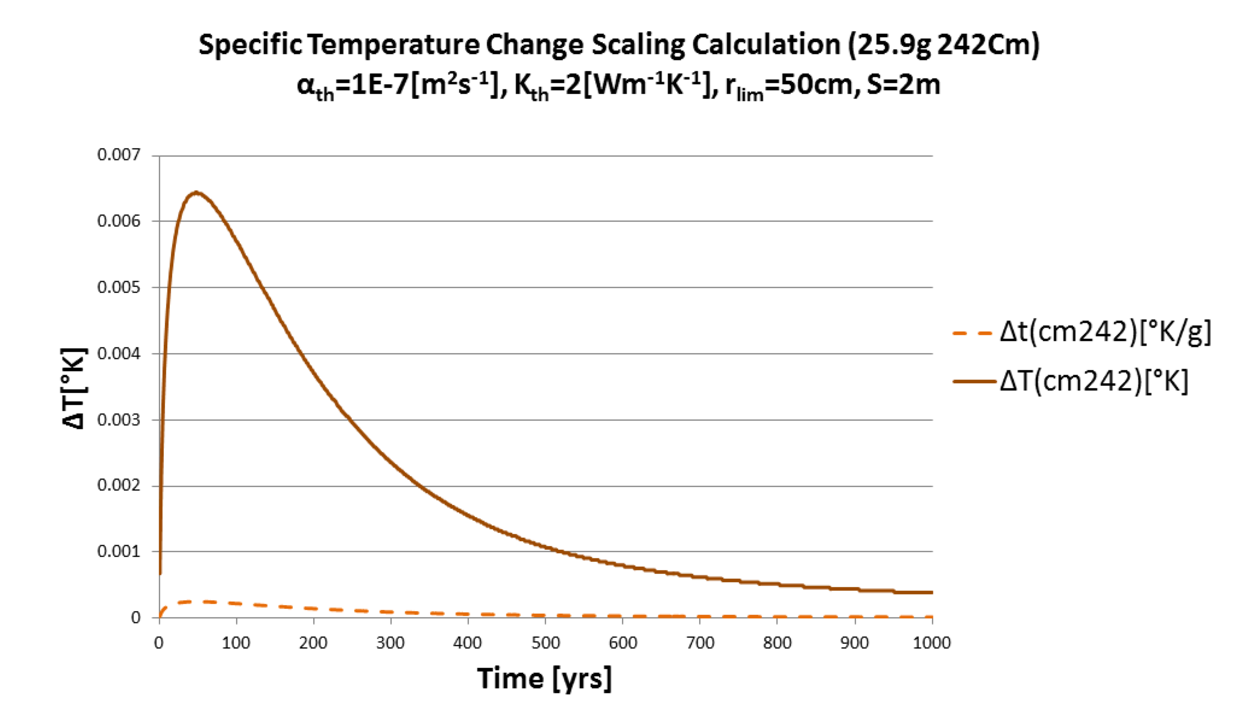
\includegraphics[width=\columnwidth]{images/CmScaling.eps}
\end{center}
\caption{As a demonstration of the calculation procedure, the temperature change 
  curve for one intial gram of $^{242}Cm$ and is scaled to represent $25.9g$, 
  approximately the $^{242}Cm$ inventory per MTHM in 51GWd burnum UOX PWR fuel. }
\label{fig:CmScaling}
\end{figure}

For an arbitrary waste stream 
composition, scaled curves calculated in this manner can be superimposed for 
each heat generating isotope to arrive at an approximate total temperature 
change at the calculation radius. 

To support this calculation in Cyder, a reference data set of temperature change 
curves, $\Delta t_i$, were calculated for high heat contributing isotopes. These 
curves were calclated as a function of specified repository spacing, $S$, heat 
limit radius, $r_{lim}$, and thermal paramters $\alpha_{th}$ and $K_{th}$. The 
total temperature change is the sum of the mass scaled curves,

\begin{align}
\Delta T &\sim \sum_{i\in H} m_i \Delta t_i(r,S,K_{th},\alpha_{th})
\intertext{where}
\Delta T &= \mbox{ total temperature change in waste }[^{\circ}K]\nonumber\\
H &= \mbox{ set of high heat isotopes }[-]\nonumber\\
m_i &= \mbox{ mass of isotope i  } [g]\nonumber\\
\Delta t_i(r,S,K_{th},\alpha_{th}) &= \mbox{ temperature change due to 1 g of i }[^{\circ}K]\nonumber
\label{superposition}
\end{align}

The use of this superposition is demonstrated in Figure 
\ref{fig:fakeArbitraryWF}.

\begin{figure}[ht!]
\begin{center}
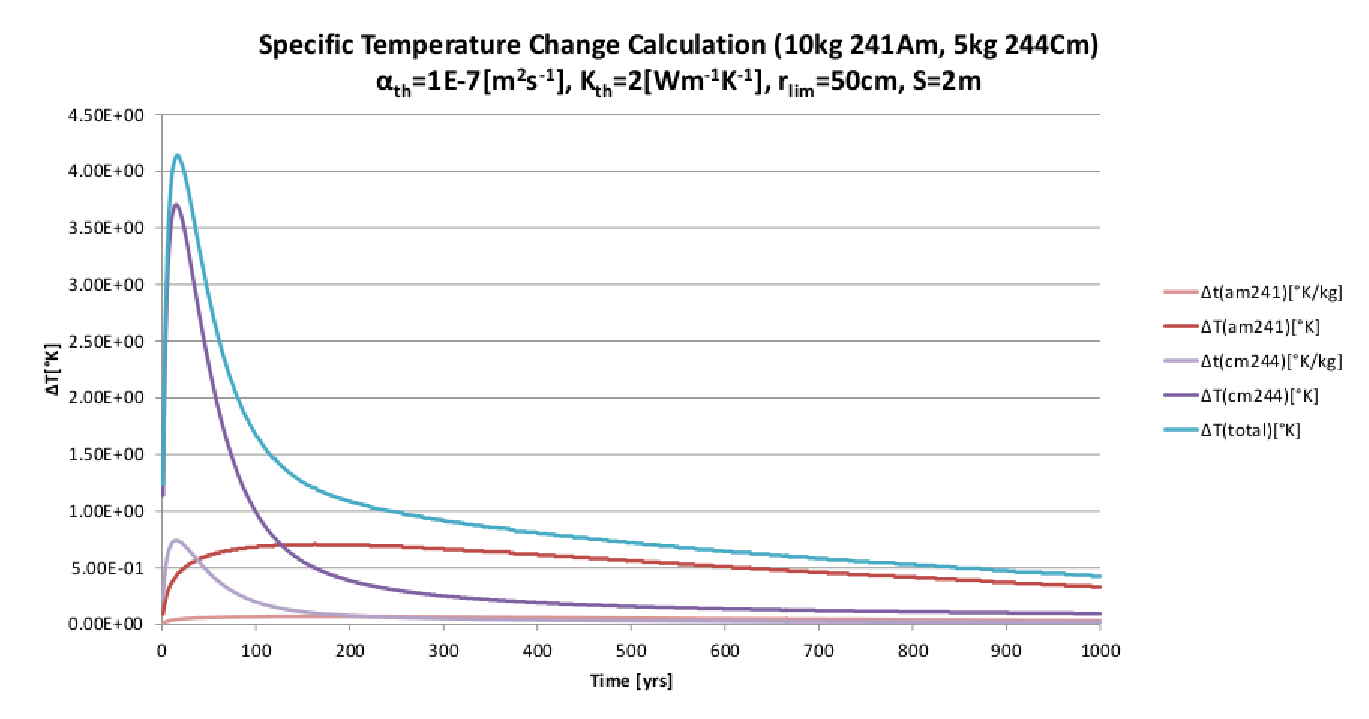
\includegraphics[width=\columnwidth]{images/fakeArbitraryWF.eps}
\end{center}
\caption{As a demonstration of the calculation procedure, scaled temperature change 
  curves for two isotopes are superimposed to achieve a total temperature 
change.}
\label{fig:fakeArbitraryWF}
\end{figure}


\begin{frame}[ctb!]
\frametitle{Specific Temperature Change Calculations}
\footnotesize{A reference data set of temperature change curves was calculated. 
Repeated runs of a detailed model over the range of values in Table 
\ref{tab:thermal_cases} determined Specific Temperature Change (STC) values over a range of thermal 
heat limit radii, $r_{lim}$, thermal diffusivity values, $\alpha_{th}$,
thermal conductivity values, $K_{th}$ and waste package spacings, $S$.

\begin{table}[ht!]
\centering
\footnotesize{
\begin{tabular}{|l|l|l|r|}
\multicolumn{4}{c}{\textbf{Thermal Cases}}\\
\hline
\textbf{Parameter} & \textbf{Symbol} & \textbf{Units} & \textbf{Value Range} \\
\hline
Diffusivity & $\alpha_{th}$ & $[m^2\cdot s^{-1}]$ & $1.0\times10^{-7}-3.0\times10^{-6}$\\
\hline
Conductivity & $K_{th}$     & $[W\cdot m^{-1} \cdot K^{-1}]$ & $0.1 - 4.5$ \\
\hline
Spacing & $S$ & $[m]$ & 2, 5, 10, 15, 20, 25, 50 \\
\hline
Radius & $r_{lim}$ & $[m]$ & 0.1, 0.25, 0.5, 1, 2, 5 \\
\hline
Isotope & $i$ & $[-]$ & $^{241,243}Am,$  \\
        & & & $^{242,243,244,245,246}Cm,$  \\
        & & & $^{238,240,241,242}Pu$  \\
        & & & $^{134,135,137}Cs$  \\
        & & & $^{90}Sr$  \\
\hline
\end{tabular}
\caption{A thermal reference dataset of \gls{STC} values as a function of each of these parameters was generated by repeated parameterized runs of the LLNL 
MathCAD model\cite{greenberg_application_2012, greenberg_investigations_2012}.}
\label{tab:thermal_cases}
}
\end{table}


}
\end{frame}


\begin{frame}[ctb!]
\frametitle{LLNL UFD MathCAD Model}
\footnotesize{
The analytic model used to populate the reference dataset was created at 
LLNL for the UFD campaign \cite{hardin_generic_2011, 
greenberg_investigations_2012, greenberg_application_2012}. It employs an 
analytic model from Carslaw and Jaeger and is \textbf{implemented in MathCAD}
\cite{carslaw_conduction_1959, ptc_mathcad_2010}.  The integral solver in the 
MathCAD toolset is the primary calculation engine for the analytic MathCAD 
thermal model, which relies on superposition of point, finite-line, and line 
source integral solutions.  
}
\end{frame}


\begin{frame}[ctb!]
\frametitle{Scaling Demonstration}
\footnotesize{

\begin{figure}[h!]
\begin{center}
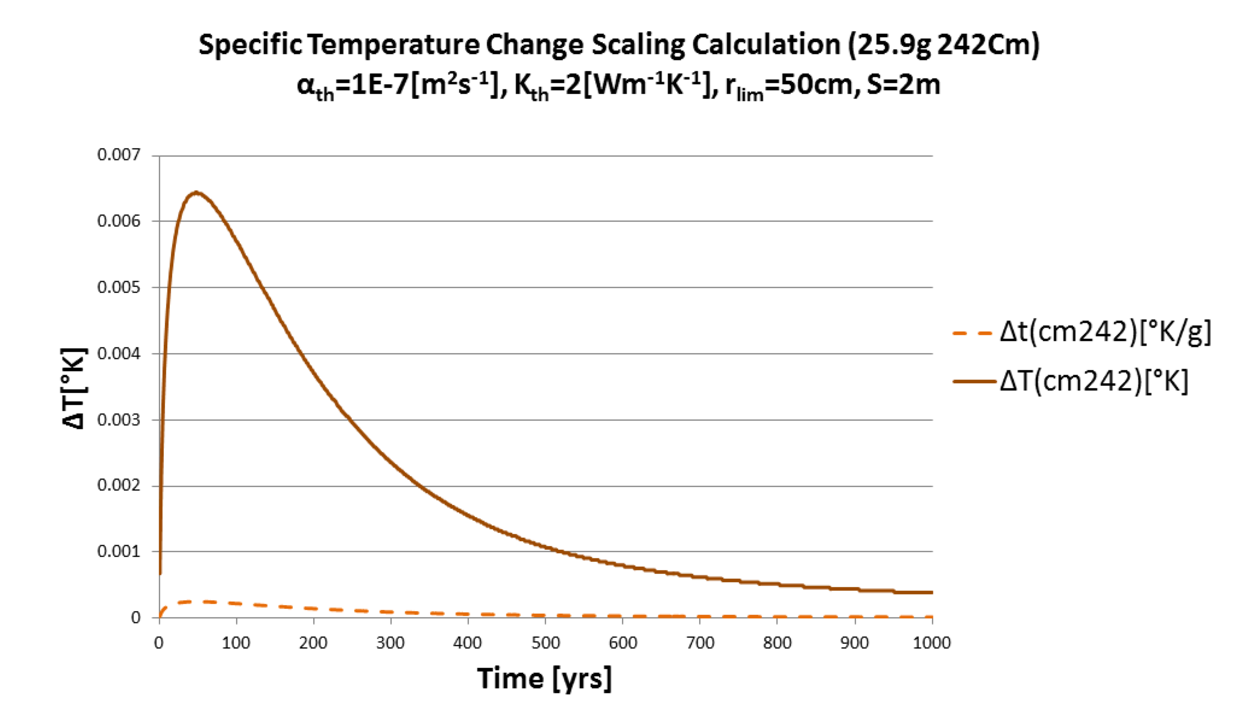
\includegraphics[width=\linewidth]{./images/CmScaling.eps}
\end{center}
\caption{As a demonstration of the calculation procedure, the temperature change 
  curve for one initial gram of $^{242}Cm$ and is scaled to represent $25.9g$, 
  approximately the $^{242}Cm$ inventory per MTHM in 51GWd burnup UOX PWR fuel. }
\label{fig:CmScaling}
\end{figure}
}
\end{frame}

\begin{frame}
\frametitle{Superposition Concept}
\footnotesize{

The supporting database was limited to some primary heat contributing isotopes 
present in traditional spent nuclear fuel, $H$, 
such that the superposition in equation \eqref{superposition} becomes 
\begin{align}
\Delta T (r_{lim},S,K_{th},\alpha_{th})&\sim \sum_{i\in H} m_i \Delta t_i(r_{lim},S,K_{th},\alpha_{th})
\label{superposition_approx}
\intertext{where}
H &= \mbox{ set of high heat isotopes }[-]\nonumber\\
S &= \mbox{ uniform waste package spacing } [m]\nonumber\\
K_{th} &= \mbox{ thermal conductivity } [W\cdot m^{-1}\cdot K^{-1}]\nonumber\\
\alpha_{th} &= \mbox{ thermal diffusivity } [m^2\cdot s^{-1}]\nonumber\\
\end{align}
}
\end{frame}


\begin{frame}
\frametitle{Superposition Demonstration}
\footnotesize{

\begin{figure}[ht!]
\begin{center}
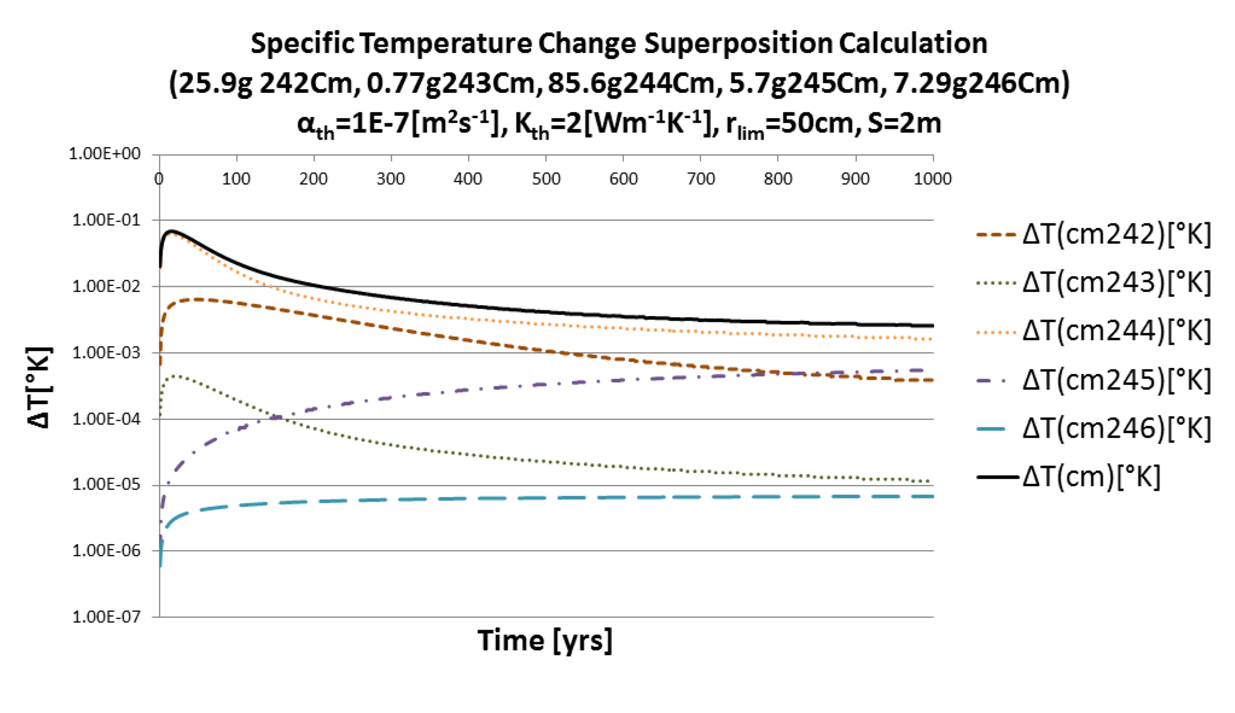
\includegraphics[width=\columnwidth]{./images/CmSuperposition.eps}
\end{center}
\caption{As a demonstration of the calculation procedure, scaled temperature change 
  curves for five curium isotopes are superimposed to achieve a total temperature 
change (note log scale).}
\label{fig:CmSuperposition}
\end{figure}

}
\end{frame}



